\documentclass{zjureport}
% =============================================
% Part 1 Edit the info
% =============================================

\newcommand{\major}{通信工程}
\newcommand{\name}{李昊}
\newcommand{\stuid}{2014210192}
\newcommand{\newdate}{2017-10-09}
\newcommand{\loc}{北邮教二509}

\newcommand{\course}{通信系统与仿真}
\newcommand{\tutor}{赵慧}
\newcommand{\newtitle}{系统传输函数零极点分析}

% =============================================
% Part 1 Main document
% =============================================
\begin{document}
\thispagestyle{empty}
\begin{figure}[h]
  \begin{minipage}{0.6\linewidth}
    \centerline{
\includegraphics[width=\linewidth]{head.jpg}}
  \end{minipage}
  \hfill
  \begin{minipage}{.4\linewidth}
    \raggedleft
    \begin{tabular*}{.8\linewidth}{ll}
      专业: & \underline\major   \\
      姓名: & \underline\name    \\
      学号: & \underline\stuid   \\
      日期: & \underline\newdate \\
    \end{tabular*}
  \end{minipage}
\end{figure}

\begin{table}[!htbp]
  \centering
  \begin{tabular*}{\linewidth}{llllll}
    课程名称: & \underline\course   & 指导老师: & \underline\tutor   & 实验名称:       &  \underline\newtitle\\
  \end{tabular*}
\end{table}

% =============================================
% Part 2 Main document
% =============================================

\section{实验要求}
	仿真比较硬解调,硬解调+软译码, 软解调+软译码
\section{总体设计}
	  \lstinputlisting[  breaklines=false ]{figures/flow.txt}

\section{工程结构}
    \lstinputlisting[language=MATLAB]{tree.txt}


\section{几个小问题}
    \lstinputlisting{questions.txt}
\section{结果分析}
    \begin{clause}
	\item 仿真
      \begin{center}
        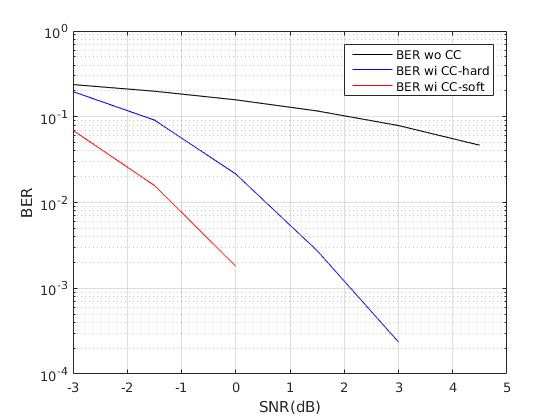
\includegraphics[width=0.6\linewidth]{main.jpg}
      \end{center}
	 \item 相对于硬解调, 加上软译码效果会提高, 如果是软解调加上软译码效果会大幅增加
	 \item 在硬解调的情况下, 加上软译码, 在同等的BER下, 可减少1.5dB的SNR
    \end{clause}
  	

\section{具体实现}
      \lstinputlisting[language=MATLAB]{code/main_c4_withCoder.m}

\end{document}
